\paragraph{Introducci\'on}
explicar separacion de partes entre oscilador y quench signal
El diseño del receptor se ha de separar en tres partes diferenciadas. En primer lugar, lo correspondiente al punto de operación del transistor, donde se trabaja con la componente DC. En segundo lugar, se desarrolla la parte de RF correspondiente al oscilador, el cual define la frecuencia de trabajo. Por último la parte correspondiente a la quench signal, encargada de gestionar el paro y arranque de la oscilación. Esta parte trabaja a una frecuencia intermedia que puede diferenciarse claramente de la parte de RF y de la componente DC.

El esquema completo del receptor se expone en la figura \ref{fig:rx}.
\begin{figure}[h]
    \centering
    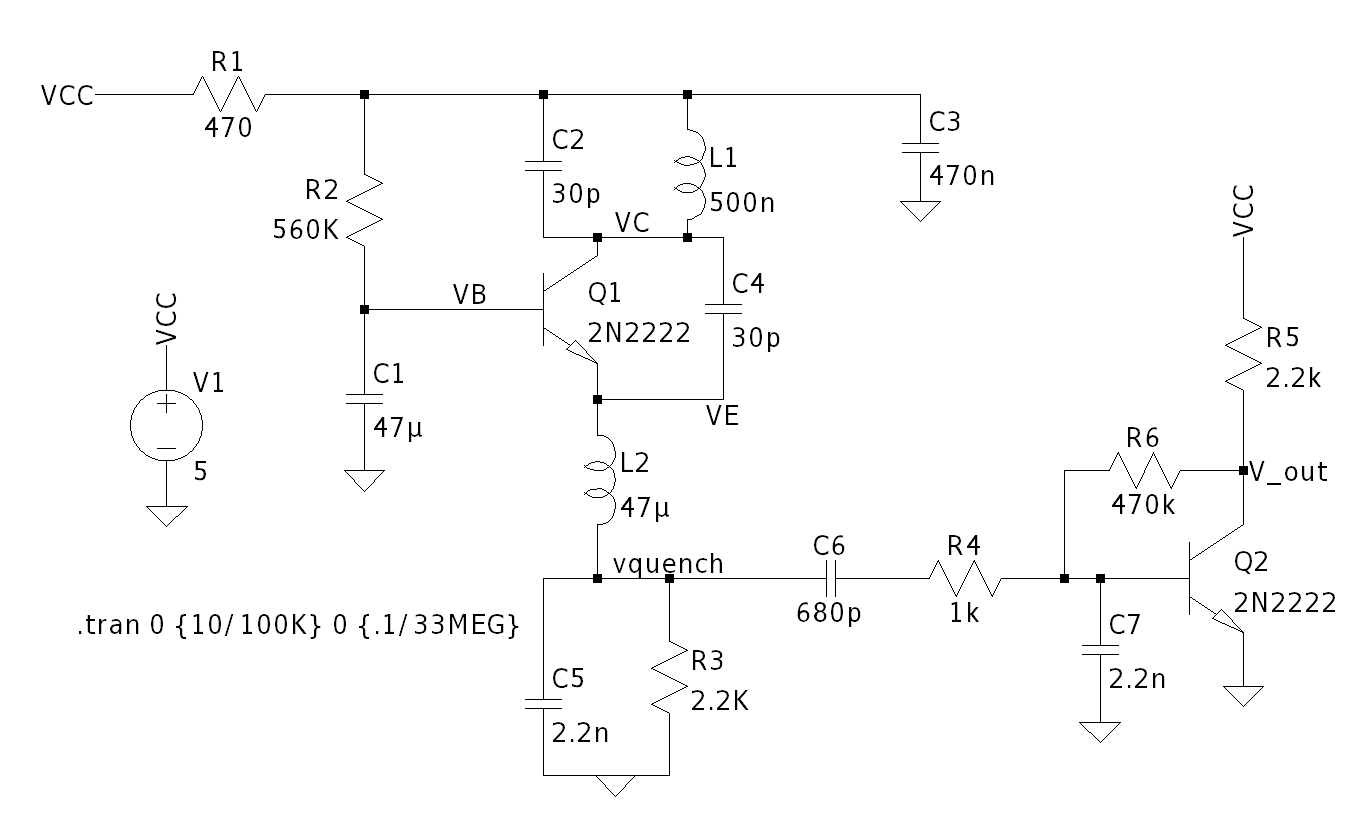
\includegraphics[scale=1, width=1\textwidth]{receptor}
    \caption{Esquema el\'ectrico del receptor}
    \label{fig:rx}
\end{figure}

\paragraph{Polarización} EXPLICAR PORQUE ESE PUNTO DE OPERACION (MENOR RUIDO POSIBLE, MENOR CONSUMO DE POTENCIA)
En este caso la estrategia para fijar el punto de operación es ligeramente distinta a como se diseña en el transmisor. El transistor debe trabajar en zona activa directa, por lo que se fijará $V_{CE} = \frac{V_{CC}}{2}$ para garantizar el mayor rango de linealidad posible. También se elige una $I_C = \SI{1}{\milli\ampere}$, en este caso para que el transistor trabaje introduciendo el mínimo ruido posible. Este hecho es importante pues, cuando el receptor se encuentra en la etapa de inicio de oscilación, un bajo nivel de ruido ayuda a aumentar la sensibilidad del receptor. Esto es debido a que la suma mínima de todos los ruidos generados por un transistor se encuentra en este rango de corriente de colector. REFERENCIA A ART OF ELECTRONICS.
Cabe recalcar que la estructura del circuito de polarización es de la forma realimentación de colector. Esta forma, provoca una realimentación negativa, que fija el punto de operación de manera más independiente a los parámetros característicos del transistor. Esta realimentación negativa debe eliminarse en corriente alterna para provocar la oscilación. La estrategia para eliminarla se verá en el apartado de pequeña señal.
Se realizan los cálculos para estimar los valores de las resistencias de polarización en función de los valores anteriormente fijados.
FIGURA AISLADA DE LA PARTE DC

\paragraph{Parte oscilador RF} IGUAL QUE EN TRANSMISOR. SMALL-SIGNAL ETC 
La estructura del oscilador en el receptor es idéntica al transmisor. Para lograr evitar la realimentación negativa provocada por la parte de polarización se coloca el condensador $C_4 = \SI{470}{\nano\farad}$, este valor es suficiente para que su impedancia para la frecuencia de RF suponga un cortocircuito a tierra. La inclusión de este condensador es imprescindible para que el circuito funcione. 
\paragraph{Modelo en pequeña señal:} Debido a que el diseño es estructuralmente igual que en el transmisor, los cálculos serán idénticos sustituyendo los valores correspondientes.
Se incluyen los valores característicos junto a las ecuaciones de interés.
En función de los valores del punto de operación obtenido, se calculan los parámetros híbridos para el receptor.

\begin{equation}
   \label{eq:result_pol1}
V_{AF} = \frac{I_{Cdata}}{h_{OEdata}} =\frac{\SI{1}{\milli\ampere}}{\SI{6}{\micro\siemens}} =  \SI{50}{\volt} 
\end{equation}
\begin{equation}
   \label{eq:result_pol2}
%\[
\begin{array}{rl} 
      \begin{array}{l}
	 h_{ib} =  \SI{8.4}{\ohm} \\
	 h_{fb} =  -0.99
      \end{array}
      &
      \begin{array}{l}
	 h_{rb} =  0.014 \\
	 h_{ob} =  \SI{6}{\micro\siemens}
      \end{array}
\end{array}
%\]
\end{equation}

\paragraph{}
El modelo en pequeña señal para las frecuencias de RF es sustancialmente igual a la parte del receptor. En la figura REF, se muestra el modelo del receptor en pequeña señal para las frecuencias de RF. L2 tiene una impedancia suficientemente grande como para considerarla circuito abierto. El objetivo del modelo es la obtención de una expresión para la frecuencia de resonancia.

\begin{figure}[h]
    \centering
    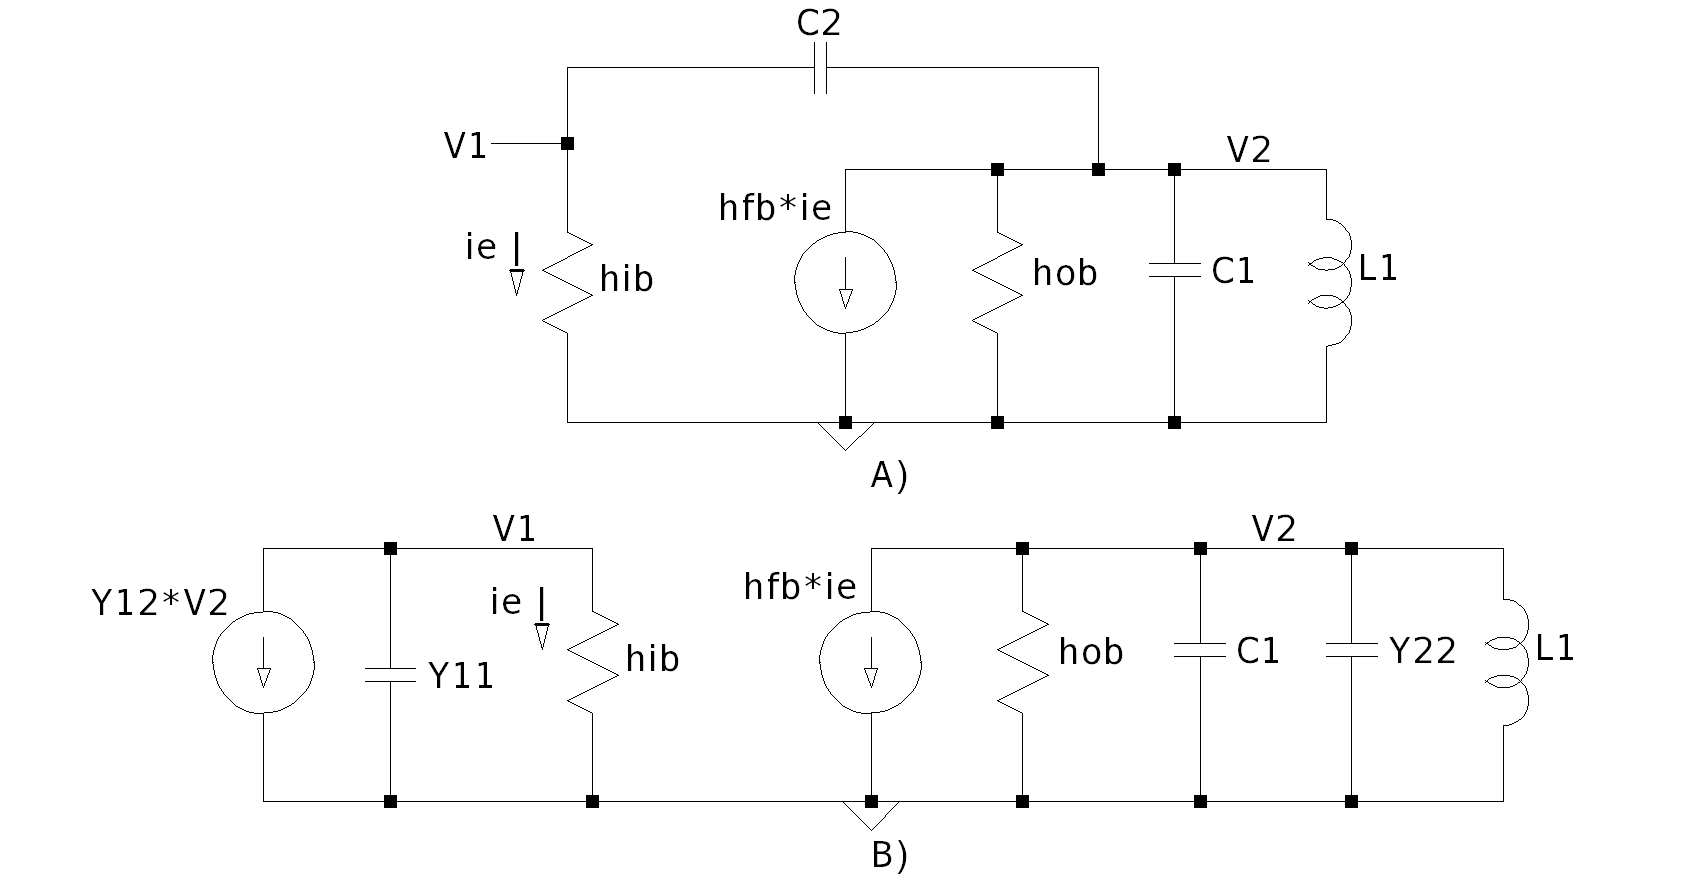
\includegraphics[scale=1, width=.8\textwidth]{small_signal_rx}
    \caption{A) Modelo en pequeña señal del bucle de oscilación para frecuencias de RF B) Modelo en pequeña señal del oscilador sustituyendo el condensador de realimentación $C_2$ por su equivalente en parámetros $Y$}
    \label{fig:ss_rx}
\end{figure}

FALTA FUNCION DE TRANSFERENCIA IGUAL QUE TX Y CALCULO DE FREQ RESONANCIA IGUAL QUE TX. RAPIDAMENTE. DECIR QUE SE ANADE CONDENSADOR VARIABLE PARA SINTONIZAR ELUDIENDO LAS DISCREPANCIAS REALES DEL CIRCUITO.
\paragraph{}
Debido a la dualidad con respecto al tx, la expresión de la función de transferencia de lazo cerrado, es idéntica al transmisor se muestra la expresión:

\begin{equation}
   \label{eq:Al_tx}
   A_l = \frac{h_{fb} \cdot C_1 \cdot s^2}{ \left( C_2+C_1 \right) \left( s \cdot h_{ib} \cdot C_2 + 1\right) \left( s^2 + s \cdot \frac{h_{ob}}{C_1 + C_2} + \frac{1}{(C_1 + C_2)\cdot L_1}\right) }
\end{equation}

\paragraph{}
Se obtiene la frecuencia de resonancia como $$\omega_0^2 = \frac{1}{L_1 \cdot (C_1 + C_2)}$$
\paragraph{}
Se obtiene el valor de la inductancia con la siguiente expresi\'on:
\begin{equation}
	\label{eq:inductance}
PONER DEL OCTAVE
\end{equation}
$$ L_1 = \SI{500}{\nano\henry} $$


\paragraph{Parte quench-signal} AISLAR CIRCUITO, REALIZAR C\'ALCULOS, L(CHOKE) R Y C
En este caso al contrario que en el receptor, la bobina de RFC no podrá ser arbitrariamente grande, pues debe permitir el paso de la frecuencia de quench pero no de la señal de RF.
%El par RC provocan la oscilación de paro y marcha del circuito, pues al realizar los cálculos, se observa que sus valores fijan el coeficiente de amortiguación del sistema. 
%i think i have now understood, the value of L2 is critical because it needs to be as large as possible to be a high impedance for rf, but an intermediate impedance to quench. This quench frequency will be always the higher possible that could be amplified in the possitive loop and at the same time can pass in the low pass filter no?
La explicación del valor de la frecuencia de quench no es algo trivial. Para poder dar explicación al fenómeno es necesario una explicación analítica antes de realizar los cálculos.
En la figura QUENCH-EXPLAIN se observa la simulación de la generación de un ciclo de oscilación y paro del mismo. Partiendo de una tensión $V_B - V_{quench} \approx \SI{0.7}{\volt}$, la oscilación comienza a generarse. Se toma como referencia $V_{quench}$ y no $V_E$ debido a que $V_E$ proporciona información tanto de las frecuencias de RF como las de frecuencia de quench, mientras que $V_{quench}$ proporciona la información de las frecuencias de interés por actuar como filtro paso bajo. 
El transistor, en configuración de base común, implica que la tensión de base $V_B$ es fija, mientras que $V_E$ varía. Mientras que la frecuencia de RF evidententemente satura y corta el transistor en numerosos ciclos por segundo, quien importa es quien corta la oscilación. A medida que la oscilación, al encontrarse dentro de un bucle de realimentación positiva, va incrementando su amplitud, la tensión media $V_{quench}$, también aumenta. En el momento que $V_{quench}$ aumenta de forma que $V_B - V_{quench} < 0.7$, el transistor se corta, matando la oscilación y provocando que la tensión $V_{quench}$ descienda, volviendo de esta forma a completar el ciclo.
\paragraph{}
Para calcular la frecuencia de quench, se debe tener en cuenta el filtro paso bajo formado por $L2, Cx, R3$ REVISAR, pero no en este caso la frecuencia de quench no se corresponde con la frecuencia de corte del filtro, ya que, el condensador no se descarga completamente en sus ciclos pues depende del transistor. 

\paragraph{Antena ??} 
a transformador de impedancias  y condensador para evitar al tocar con mano. Si no se hace explicar el acople magnetico con las bobinas

\paragraph{Resultado simulaci\'on} Se muestran las medidas simuladas de tension de mayor inter\'es con la nomenclatura de la figura FIG RF
captura de oscilacion de rf, v en rc y vout
captura con senal de entrada vout cambia de frecuencia

\paragraph{}
En el apartado de simulación trata de obtener una represaentación gráfica de lo desarrollado anteriormente sobre el receptor. Por ello, en la figura REF se observan los puntos de interés del circuito como son $V_C$, $V_{quench}$ y $V_{B}$, además de añadir la diferencia$V_B - V_{quench}$ como $V(B,quench)$. Estas cuatro medidas son suficientes para entender el ciclo de paro y marcha del transistor.
\paragraph{}
Como se puede observar en la figura \ref{fig:simrx_zoom}, a medida que se construye la oscilación, el valor medio de la tensión de $V_{C}$, es decir $V_{quench}$, aumenta hasta que finalmente, la diferencia $V_B - V_{quench} < \SI{.7}{\volt}$ hace desaparecer la oscilaci\'on. Este corte provoca que el valor medio de $V_C$ descienda, y por tanto $V_{quench}$, provocando finalmente que la diferencia $V_B - V_{quench} > \SI{.7}{\volt}$ reactivando al transistor y reiniciando el ciclo de oscilaci\'on.

\begin{figure}[h]
    \centering
    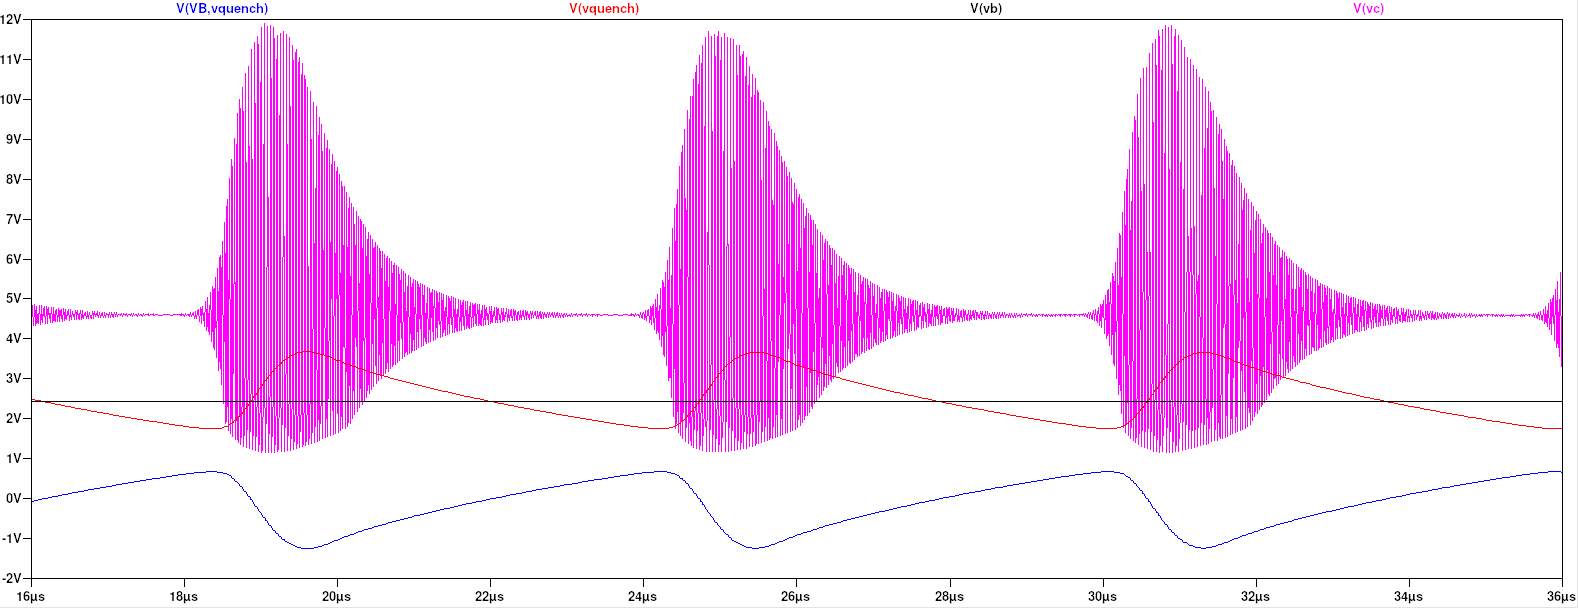
\includegraphics[scale=1, width=1\textwidth]{simrx_zoom}
    \caption{Simulación de puntos de interés en varios ciclos ampliados}
    \label{fig:simrx_zoom}
\end{figure}

\paragraph{}
Se añade también, en la figura \ref{fig:simrx_vout}, la forma de onda de la tensión de salida $V_{out}$, que es la señal de entrada al microcontrolador atmega328p, el cual se encargará de demodular la señal. Esta señal debe ser una señal digital entre \SI{0}{\volt} y \SI{5}{\volt}.
\begin{figure}[h]
    \centering
    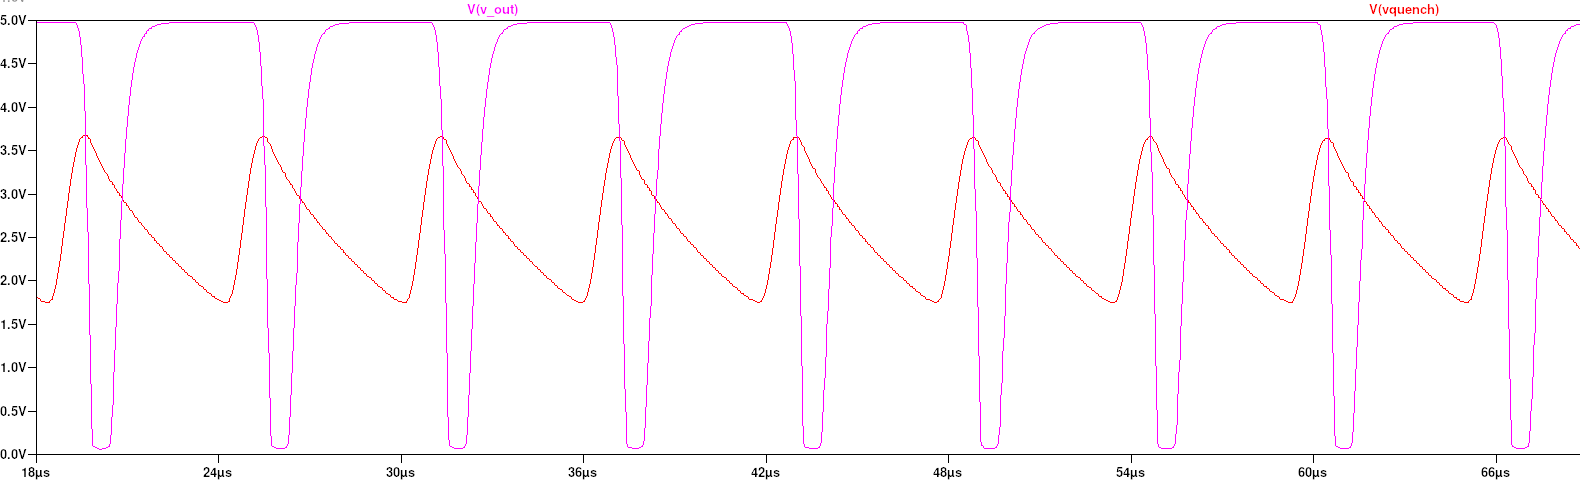
\includegraphics[scale=1, width=1\textwidth]{simrx_vout}
    \caption{Simulación de $V_{out}$ junto a $V_{quench}$}
    \label{fig:simrx_vout}
\end{figure}

\paragraph{Resultado práctico} En este caso se muestran las medidas tomadas en el apartado de simulacion, esta vez tomadas en el circuito real. Las medidas se toman usando un osciloscopio. 
La configuración es la misma que en el en el apartado REF del transmisor. En este caso al disponer de dos canales se muestran en la figura REF los puntos $V_{quench}$ (rojo) y $V_{C}$ (amarillo).

lo mismo que en simulacion pero capturas de osciloscopio
% situacion en el circuito (imagen bloque) y partes, enumeracion partes
% explicacion recepcion directa amplificando senal de RF y demodulando con filtro, posteriormente etapa de smith triger que se 
% manda al microcontrolador y detecta el canal. 
% \subsubsection{sintonizaci\'on y etapa de par Darlington}
% El circuito sintonizado que consigue la sensibilidad necesaria para captar la señal modulada proviniente del transmisor se consigue mediante un filtro paso banda sintonizado a la frecuencia de portadora. La corriente en la bobina $L_1$ producida por el campo electromagnético recibido, se amplifica notablemente a trav\'es de la etapa darlington, la cual, se encuentra polarizada con un $V_{CE}$ suficientemente bajo como para provocar la saturaci\'on del transistor ante la m\'inima intensidad de corriente en su entrada.
% \paragraph{Polarizaci\'on:} el par darlington debe ser lo suficientemente sensible como para poder detectar la corriente inducida en la bobina de recepci\'on, por lo que $I_B \approx \SI{28}{\nano\ampere}$
% \paragraph{Modelo en pequeña señal:} El objetivo de este apartado es el cálculo de la ganancia de la corriente de entrada con respecto a la tensión de salida de la etapa, y su impedancia de salida
% \subsubsection{Etapa en colector com\'un}
% Esta etapa actúa como un adaptador de impedancias de tal forma que la tensión de salida de la etapa darlington ataque a una impedancia de entrada alta para evitar pérdidas, mientras que la impedancia de salida de la etapa en colector común es baja y de ganancia en tensión similar a la unidad. A esta configuración se la conoce como \textit{"voltage buffer"}.
% \paragraph{Polarizaci\'on:} Se debe fijar una corriente de base del orden de la corriente que pueda proporcionar la etapa anterior, unos \SI{30}{\micro\ampere}. De forma an\'aloga a los anteriores apartados, se calcula el punto de operaci\'on para los valores del esquem\'atico, figura \ref{}
% \subsubsection{Amplificador de tensi\'on y filtro paso bajo}
% \subsubsection{comparador Smith triger}
% \subsubsection{Demodulaci\'on digital}
% demodulaci\'on digital a tr\'aves del microcontrolador se expondra en la sección 

